\documentclass[12pt]{exam}
\usepackage[utf8]{inputenc}

\usepackage[margin=.5in]{geometry}
\usepackage{amsmath,amssymb}
\usepackage{multicol}
\usepackage{datetime}
\usepackage{graphicx}
\usepackage{xcolor}
\usepackage{calc}

\graphicspath{ {./images/} }

\usepackage{minted}
\definecolor{dgreen}{HTML}{049101}
\definecolor{Lblue}{HTML}{2561ba}
\definecolor{mygray}{gray}{0.9}

\newcommand{\ansb}[1]{\textcolor{dgreen}{\textbf{#1}}}
\newcommand{\ans}[1]{\textcolor{dgreen}{#1}}

\newcommand{\alink}[2]{\href{#1}{\underline{\textcolor{Lblue}{Reference: #2}}}}

% \newcommand{\vline}[2]{\begin{center}\noindent\rule{#1cm}{#2pt}\end{center}}
\newcommand{\fline}{\begin{center}\noindent\rule{18cm}{0.75pt}\end{center}}

% \newcommand{\ansbox}[1]{\parbox{\textwidth}{\textbf{Answer}:\\ {#1}}}

% \newcommand{\ansbox}[1]{
% \noindent\fbox{%
%     \parbox{\textwidth}{#1}%
% }}

\newcommand{\ansbox}[1]{
\textcolor{dgreen}{\textbf{Answer:}}\\
\noindent\colorbox[gray]{0.90}{%
    \parbox{\textwidth - 12 \fboxsep}{\ans{#1}}%
}}

\usepackage{tikz}
\usetikzlibrary{graphs,arrows.meta}


\pagestyle{head}
\firstpageheader{}{}{}
\runningheader{\class}{\examnum\ - Page \thepage\ of \numpages}{\examdate}
\runningheadrule

\newcommand{\class}{3013 - Alorithms}
\newcommand{\term}{Spring 2020}
\newcommand{\examnum}{Exam 1}
\newcommand{\examdate}{\today}
\newcommand{\timelimit}{80 Minutes}
\newcommand{\seperate}{\begin{center}\noindent\rule{18cm}{0.75pt}\end{center}}



\begin{document}

\noindent
\begin{tabular*}{\textwidth}{l @{\extracolsep{\fill}} r @{\extracolsep{6pt}} l}
    \textbf{\class} & \textbf{Name:} & \makebox[2in]{\hrulefill}\\
    \textbf{\term} &&\\
    \textbf{\examnum} &&\\
    \textbf{\examdate} &&\\
    % \textbf{Time Limit: \timelimit} & Teaching Assistant & \makebox[2in]{\hrulefill}
\end{tabular*}\\
\rule[2ex]{\textwidth}{2pt}

\renewcommand{\arraystretch}{1.25}
\begin{tabular}{ | p{8cm} | p{8cm} | }
    \hline
    \multicolumn{2}{|c|}{\textbf{READ THESE INSTRUCTIONS}}\\
    \hline
    Use pencil only                                                & Write name at the top of all pages turned in.     \\
    \hline
    Staple pages together at the top left corner.                  & Illegible handwriting will lose points.           \\
    \hline
    Make sure your pages are in order when stapled.                & All questions written in order on paper provided. \\
    \hline
    Write answers on the paper provided, not directly on the test. & Indentation matters. Keep code aligned correctly. \\
    \hline
    \multicolumn{2}{|c|}{ Lists of items should be written vertically not horizontally.} \\
    \hline
    \multicolumn{1}{|c|}{GOOD}                                     & \multicolumn{1}{|c|}{BAD}                         \\

    \includegraphics[scale=.5]{./graphics/ex_ans_list}             &
    \includegraphics[scale=.5]{./graphics/ex_ans_list_bad}\\
    \hline
    \multicolumn{2}{|c|}{\textbf{Failure to comply will result in loss of letter grade.}}\\
    \hline
    \multicolumn{2}{c}{This exam is \numpages\ pages (without cover page) and \numquestions\ questions. Total of points is \numpoints.}\\
\end{tabular}
\begin{center}

    Grade Table (don't write on it)\\
    \addpoints
    \gradetable[v][questions]
\end{center}

\noindent
\rule[2ex]{\textwidth}{2pt}
\clearpage



\begin{questions}

    \question[5]Flip back to the cover page. Write your name there.

    %######################
    \seperate
    %######################

    \question[20]List the complexities from fastest to slowest.

    \begin{tabular}{ c  c  c  c  c  c  c  c c }
        \multicolumn{8}{c}{Complexity Choices} \\
        $O(n!)$ & $O(2^n)$ & $O(1)$ & $O(n\ lg\ n)$ & $O(n^2)$ & $O(n^n)$ & $O(n)$ & $O(log\ n)$ & None of These \\
    \end{tabular}\\


    \ansbox{
        \begin{enumerate}
            \item $O(1)$
            \item $O(log\ n)$
            \item $O(n)$
            \item $O(n\ lg\ n)$
            \item $O(n^2)$
            \item $O(2^n)$
            \item $O(n!)$
            \item $O(n^n)$
        \end{enumerate}
    }




    %######################
    \seperate
    %######################

    \question[20] Given the following binary tree:

    \includegraphics[scale=.35]{graphics/tree_again.png}

    \ansbox{
    \begin{tabular}{ c  l  l}
        1 & What is the height of this tree?                & 5 or 6              \\
        2 & What is the root of this tree?                  & 33                  \\
        3 & How many leaves does this tree have? List them. & 5,12,19,25,30,37,53 \\
        4 & How many descendants does 23 have?              & 9                   \\
        5 & How many siblings does 23 have?                 & 1                   \\
        6 & Who is the predecessor of 23?                   & 19                  \\
        7 & Who is the successor of 23?                     & 25                  \\
    \end{tabular}
    }

    %######################
    \seperate
    %######################
\clearpage
    \question[20]Assign the correct complexity to each item below.

    \begin{tabular}{ c  c  c  c  c  c  c  c c }
        \multicolumn{8}{c}{Complexity Choices} \\
        $O(n!)$ & $O(2^n)$ & $O(1)$ & $O(n\ lg\ n)$ & $O(n^2)$ & $O(n^n)$ & $O(n)$ & $O(log\ n)$ & None of These \\
    \end{tabular}
    \\
    \ansbox{
    \begin{tabular}{ c  l  l}
        1  & Inserting an element into a balanced binary search tree. & $O(log\ n)$ \\
        2  & Finding an element in a list.                            & $O(n)$      \\
        3  & Finding an element in an ordered list.                   & $O(n)$      \\
        4  & Removing an element from a binary heap.                  & $O(log\ n)$ \\
        5  & Finding an element in a binary search tree.              & $O(log\ n)$ \\
        6  & Adding an element to a binary heap.                      & $O(log\ n)$ \\
        7  & Building a binary heap given an array of values.         & $O(n)$      \\
        8  & Building a binary heap given a linked list of values.    & $O(log\ n)$ \\
        9  & Remove an item from a linked list of values.             & $O(1)$      \\
        10 & Insert an item into an ordered linked list of values.    & $O(n)$      \\
    \end{tabular}
    }
    \seperate

    \question[10] \textbf{Heapify}: Describe what it does, and why it is significant. Be thorough.

    \ansbox{
    \begin{itemize}
        \item \textbf{Heapify} takes an array of values, and turns it into a heap (min or max depending on need). 
        \item It is significant because it can accomplish creating a heap faster than inserting items into an empty 
    heap 1 item at a time. 
        \item If we insert $n$ items into a heap at a cost of $O(lg\ n)$ per insert, we can build a heap
    with a cost of $O(n\ lg\ n)$. Not bad, but using \textbf{Heapify} only costs us $O(n)$!! 
        \item How does it do this in linear time? Well we could prove it by solving a summation and doing 
        some substitutions and removals of constants etc. (https://www.growingwiththeweb.com/data-structures/binary-heap/build-heap-proof/), OR we can just understand 
        that we don't need to process the entire array of values because the entire bottom row of our tree (more than half the nodes) are leaf's. And by processing only the top half of the array (swapping as necessary with children) we end up with an array in heap order. Yes, some values may need to be swapped more than once, but this also is shown to be a "constant" time cost, which can be ignored :/  
    \end{itemize}
    }

    %######################
    \seperate
    %######################
\clearpage
    \question[15] Write a pseudo code implementation for deleting a node from a binary search tree. \\
    \\
    \noindent\fcolorbox{black}{mygray}{%
        \begin{minipage}{\dimexpr1\textwidth-2\fboxrule-2\fboxsep\relax}
            \textbf{Answer 1}:\\
            \begin{itemize}
                \item Assuming we find the node with the "key" in it that needs deleting.
                \item \textbf{1) No children:} Simply delete the node with the key. Set parents pointer to $NULL$.
                \item \textbf{2) One child:} Delete the node with the key, and have the parent take over its single child.
                \item \textbf{3) Two children:} this is indeed the "complicated" case.
                      \begin{enumerate}
                          \item Find the rightmost node of the left child (or the leftmost node of the right child) of the node with key in it.
                          \item Swap the found value with node that needs deleting (its either its predecessor or successor so it doesn't "break" the order in the tree.
                          \item Delete the node it was swapped into since it should be an instance of case 1 or case 2
                      \end{enumerate},

            \end{itemize}
        \end{minipage}}


    \textbf{Answer 2}:\\
    \begin{minted}
[
frame=lines,
framesep=2mm,
baselinestretch=1.2,
% bgcolor=LightGray,
fontsize=\footnotesize,
linenos
]
{c++}
    if ( key not in BST )
    {
       return;         // Nothing to delete
    }

    if ( key has no children )              //     x            x
    {                                       //    / \    ==>   /
       delete key from keys parent;         //   y   k        y
       return;                              //
    }

    if ( k has 1 child )                          //     x            x
    {                                             //    / \    ==>   / \
       make keys parent point to keys child;      //   y   k        y   z
       return;                                    //        \
    }                                                        z

    /* k has 2 subtrees - TOUGH */

   //(1)  find the successor of key:
   //         go right once
   //       go left all the way down
   //
   // (2) Replace key with keys successor;
   //
   // (3) Make the successors parent point to the successors right subtree;  
\end{minted}


    %######################
    \seperate
    %######################

    \question[10] Take the values from the max heap below and draw an array that would represent this tree.

    Put the answer on your answer sheet using something similar to:  \includegraphics[scale=.35]{graphics/empty_array.png}

    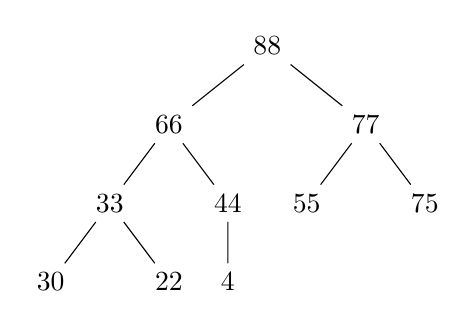
\begin{tikzpicture}[level distance=1cm,
            level 1/.style={sibling distance=2.5cm},
            level 2/.style={sibling distance=1.5cm}]
        \node {88}
        child {node {66}
                child {node {33}
                        child {node {30}}
                        child {node {22}}
                    }
                child {node {44}
                        child {node {4}}
                    }
            }
        child {node {77}
                child {node {55}}
                child {node {75}}
            };
    \end{tikzpicture}
    \\
    \noindent\fcolorbox{black}{white}{%
        \begin{minipage}{\dimexpr.75\textwidth-2\fboxrule-2\fboxsep\relax}
            \\
            \textbf{Answer}:\\
            \\
            \begin{tabular}{|c|c|c|c|c|c|c|c|c|c|c|}
                \hline
                x & 88 & 66 & 77 & 33 & 44 & 55 & 75 & 30 & 22 & 4  \\
                \hline
                0 & 1  & 2  & 3  & 4  & 5  & 6  & 7  & 8  & 9  & 10 \\
                \hline
            \end{tabular}
        \end{minipage}}

    %######################
    \seperate
    %######################

    \question[15] Given a sequence of numbers: 19, 6, 8, 11, 4, 5
    \begin{parts}
        \part[5] Draw a binary min-heap (in a tree form) by inserting the above numbers reading them from left to right
        \part[5] Show a tree that can be the result after the call to deleteMin() on the above heap
        \part[5] Show a tree after another call to deleteMin()
    \end{parts}

    %######################
    \seperate
    %######################


    \question[30] List vs Array based data structures. Given a statement below, choose:\\
    \textbf{List}, \textbf{Array}, \textbf{Both}, \textbf{None}\\
    to indicate what the statement is implying.

    \begin{tabular}{ c  c  c  c }
        \textbf{Choices:} List & Array & Both & None \\
    \end{tabular}

    \renewcommand{\theenumi}{\Alph{enumi}}
    \begin{enumerate}
        \item Directly access element in this structure.
        \item Bounded by size.
        \item Easy to insert and delete from.
        \item Easy to implement.
        \item More overhead.
        \item Can be sorted.
        \item Must be allocated in the heap.
        \item Expensive to resize.
        \item Grows and shrinks easily.
        \item Binary search can be performed on this.
        \item Easily access each element in this structure.
        \item Cannot be allocated in the heap.
        \item Must be statically declared.
        \item Items added to front or rear.
        \item Easier to delete from middle of structure.
        \item Can be used to represent a binary tree.
    \end{enumerate}


    \question[5] Give a pre-order / post-order /in-order traversal of the following tree:

    \includegraphics[scale=.5]{graphics/tree_traverse.png}

    \question[20]  Stack based memory VS Heap based memory.
    \begin{parts}
        \part[10]Pros and cons of a Stack
        \part[10]Pros and cons of the Heap
    \end{parts}

    \question[20]
    \begin{parts}
        \part[10] Draw the resulting binary search tree by inserting the following values from left to right: \textbf{19, 6, 8, 11, 4, 13, 5, 27, 43, 49, 31, 25}
        \part[10] Delete \textbf{19} from the binary search tree in part (a) using a standard removal algorithm for binary search trees. Draw the TWO potential binary search trees that you can end up with.
    \end{parts}

    %######################
    \seperate
    %######################

    \question[20] You are attending a party with $n$ other people. Each other person $i$ arrives at the party at some time
    $s_i$ and leaves the party at some time $t_i$ (where $s_i < t_i$). Once a person leaves the party, they do not return.
    Additionally, each person $i$ has some coolness $c_i$. At all times during the party, you choose to talk to the coolest person currently at the party. (All coolness values are distinct.) If you are talking to someone, and someone else cooler arrives at the party, you leave your current conversation partner and talk to the new person. If the person you are talking to leaves the party, you go talk to the coolest person remaining at the party. (This might or might not be a person with whom you have already talked.) You are the first to arrive at the party and the last to leave. Additionally, you are the most popular
    person at the party, so everyone wants to talk with you.

    Describe a data structure which allows you to decide in $O(1)$ time to whom you should talk at any moment. You should be able to update this data structure in $O(log n)$ time when someone arrives or leaves.

    \question[5]Write your name on your answer sheets.

\end{questions}
\end{document}